\chapter{Productivity mobile applications analysis}
\label{chap:apps}
Let's consider the most popular productivity mobile applications on the iOS devices in order to understand market and how does these application solve the problem of effective task management.

\section{Popular applications and their description}

\textbf{Habit List.} \url{http://habitlist.com/} Habit List is an application to create good habits and break unhealthy ones. Habit List allows users to track habits and provide visual representations on progress. This encourages more success by seeing the results of hard work or lack thereof. The app is quick to load and the design is simple but effective. It’s essentially a list of items that a user would like to complete on a certain schedule. Each habit’s status is communicated through a green or red indicator. Inside the colored indicator is the streak of days that a habit has been completed or not been completed.

\begin{figure}
   \centering
	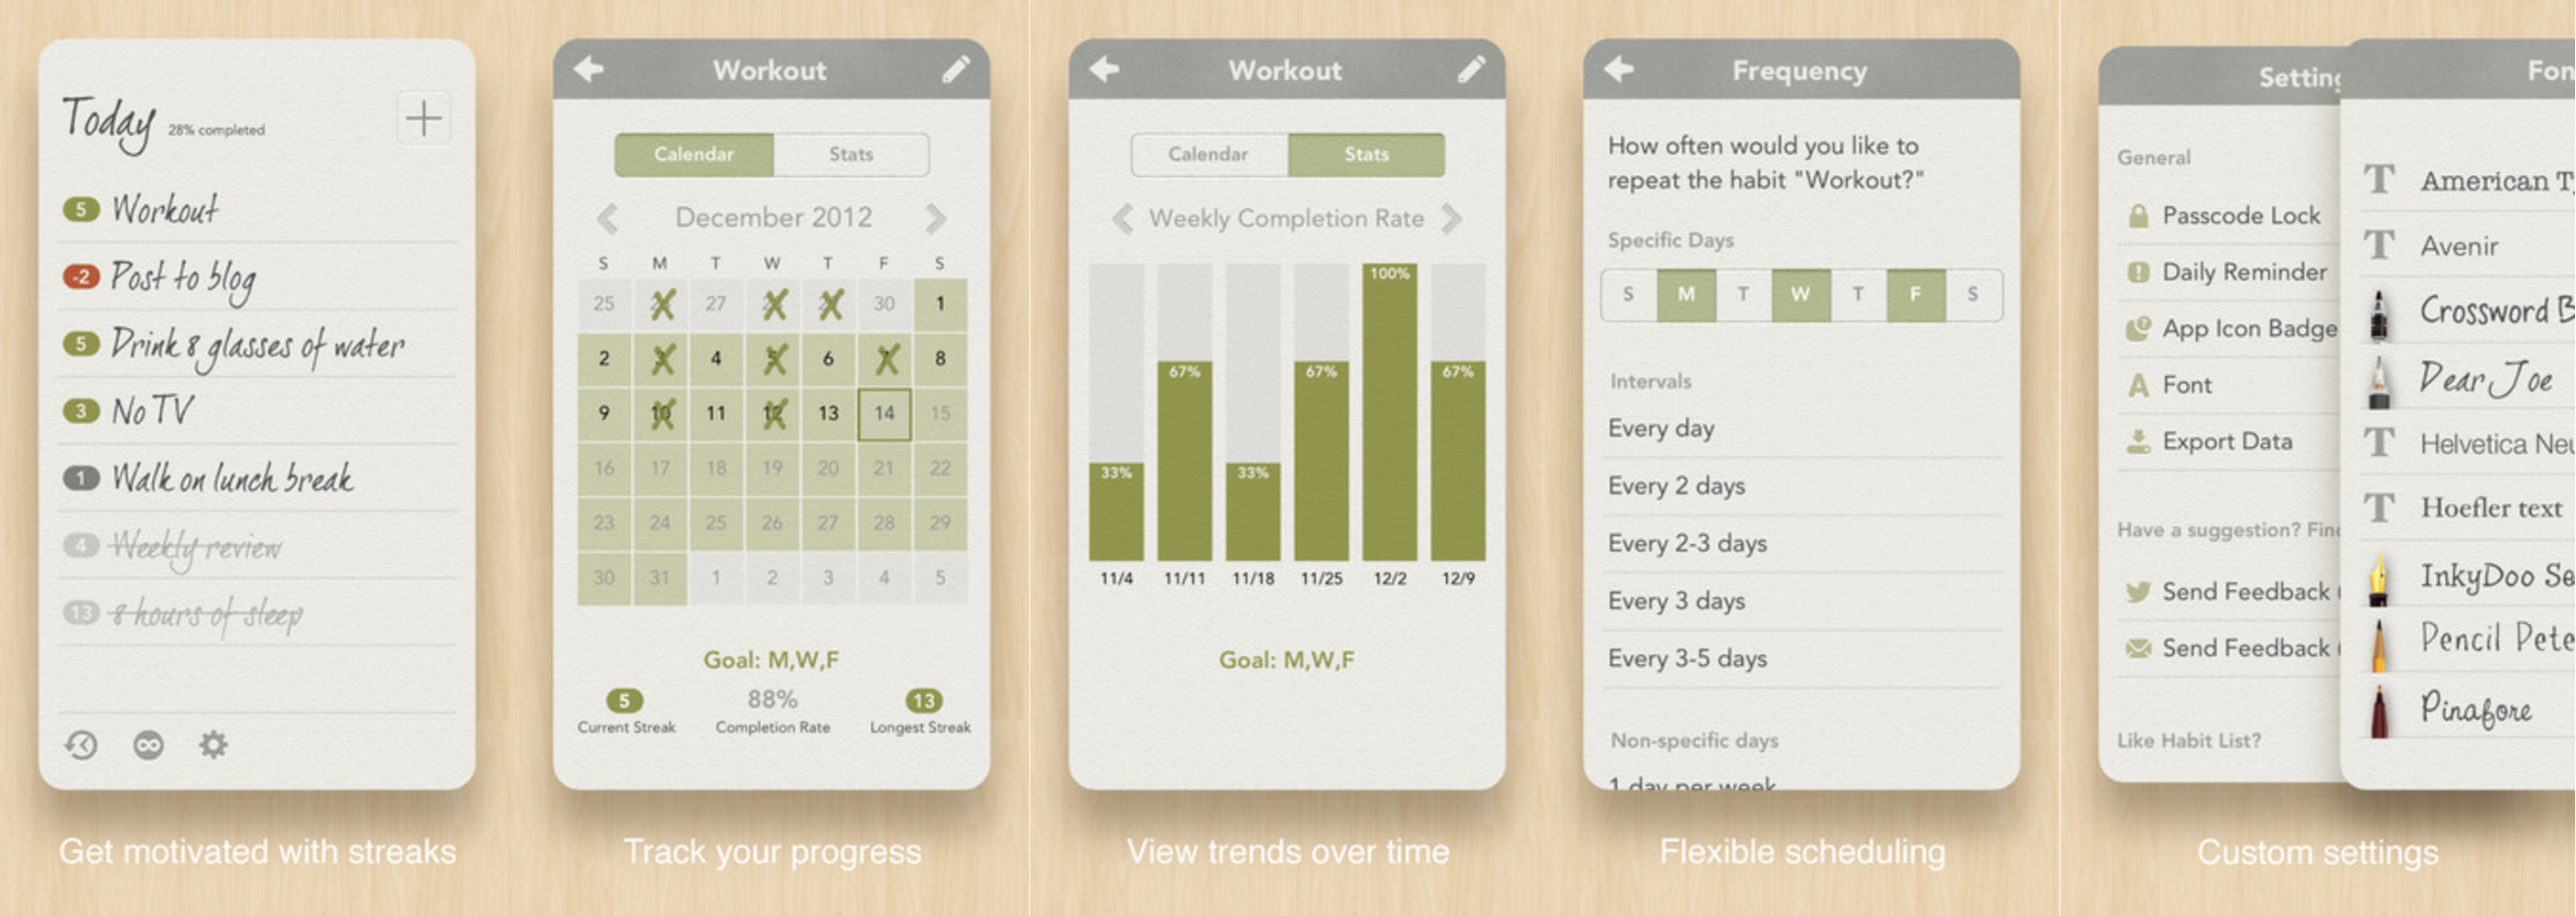
\includegraphics[width=0.9\textwidth]{resources/habit-list.pdf}
	\caption[Habit List]{Habit list}
\end{figure}

\textbf{Carrot.} \url{http://meetcarrot.com/} Carrot encourages users to get tasks done in a timely matter and they're rewarded with points that lead to unlockable features. But if they don't accomplish tasks then the app will get angry.

\begin{figure}
   \centering
	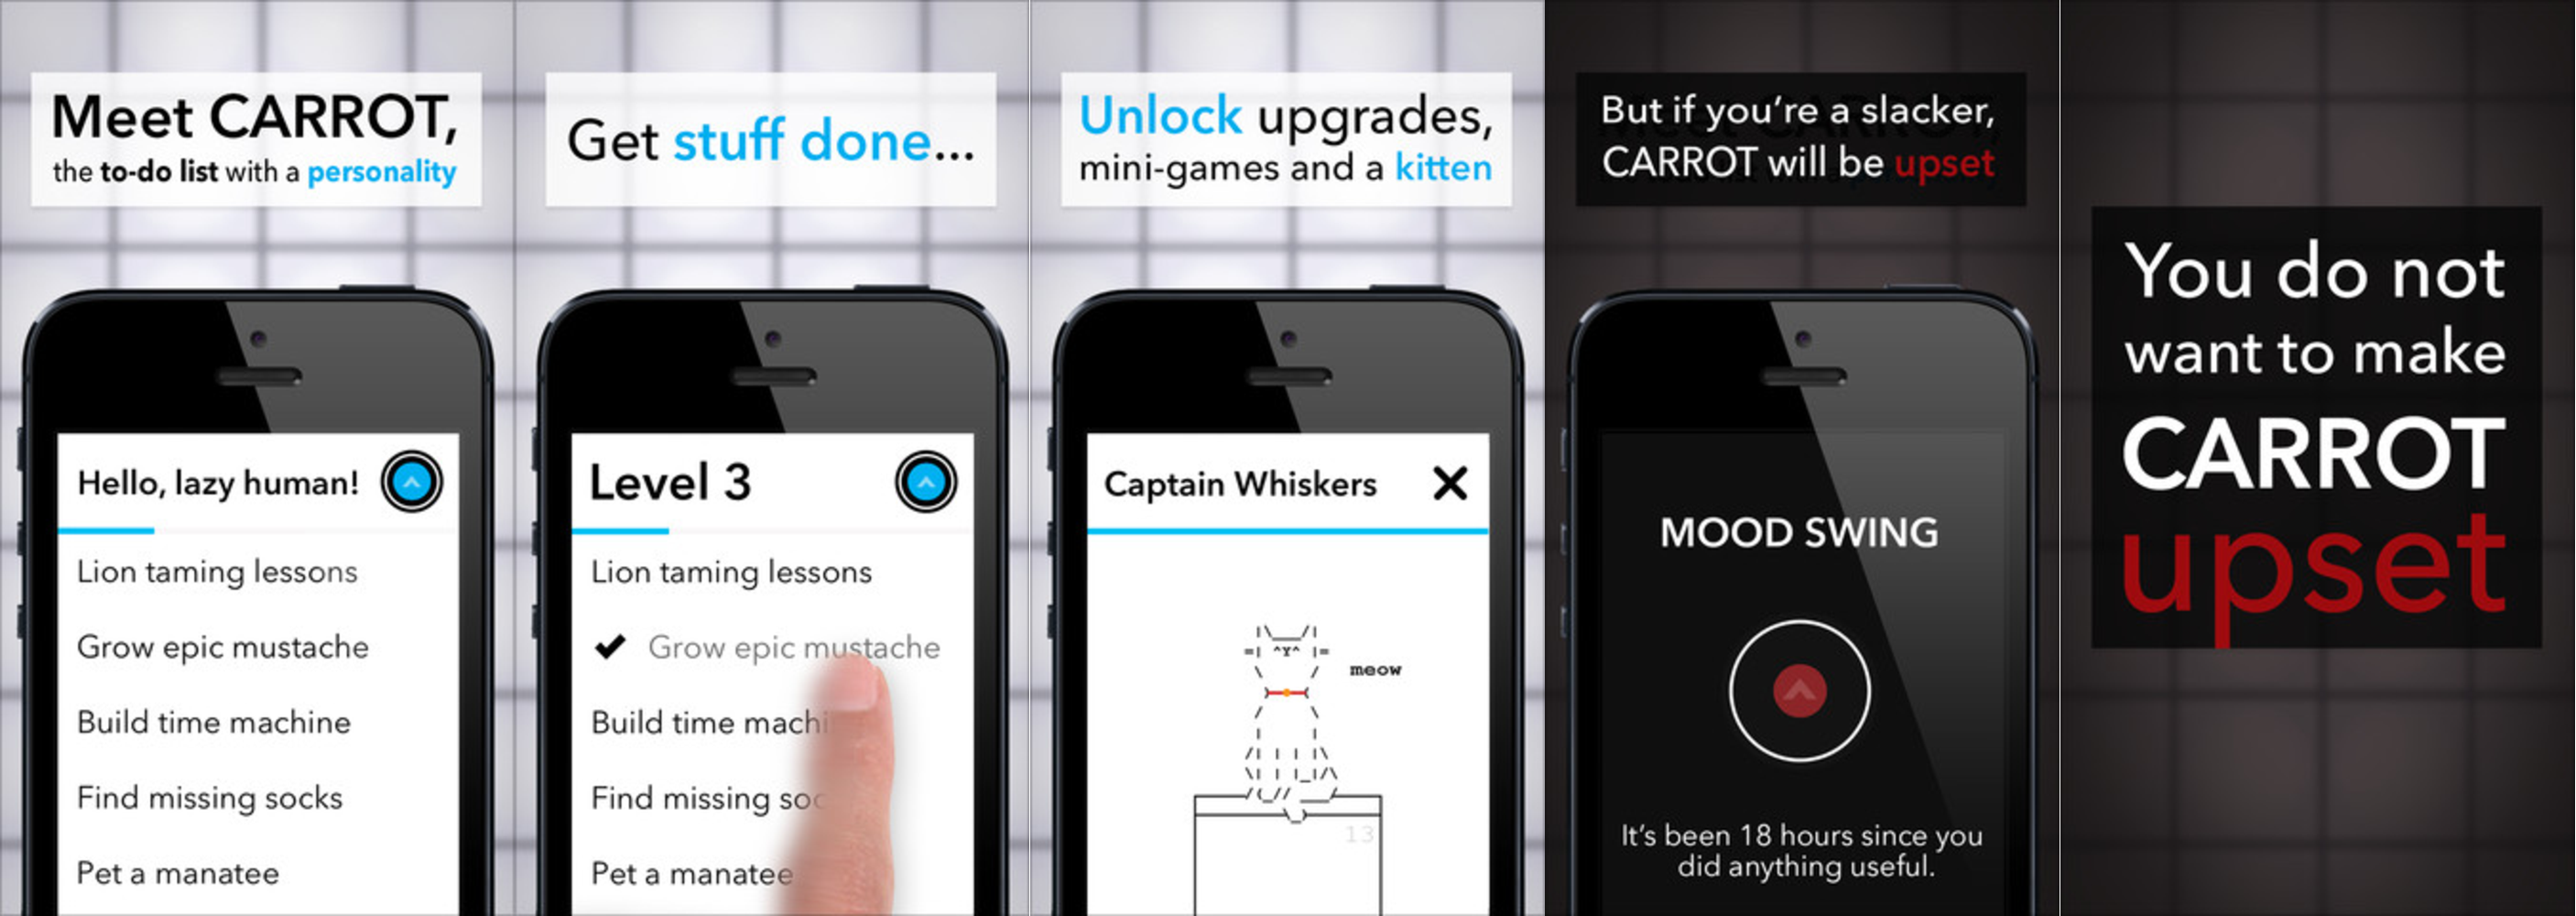
\includegraphics[width=0.9\textwidth]{resources/carrot.pdf}
	\caption[Carrot]{Carrot}
\end{figure}

\textbf{Clear.} \url{http://www.realmacsoftware.com/clear/} Clear uses the hierarchy of color, which is utilized to represent priority within the app. The idea is that to-do list becomes a heat map, where the warmest areas (i.e. the ones with the strongest shade of red) are the tasks should be attended first.

\begin{figure}
   \centering
	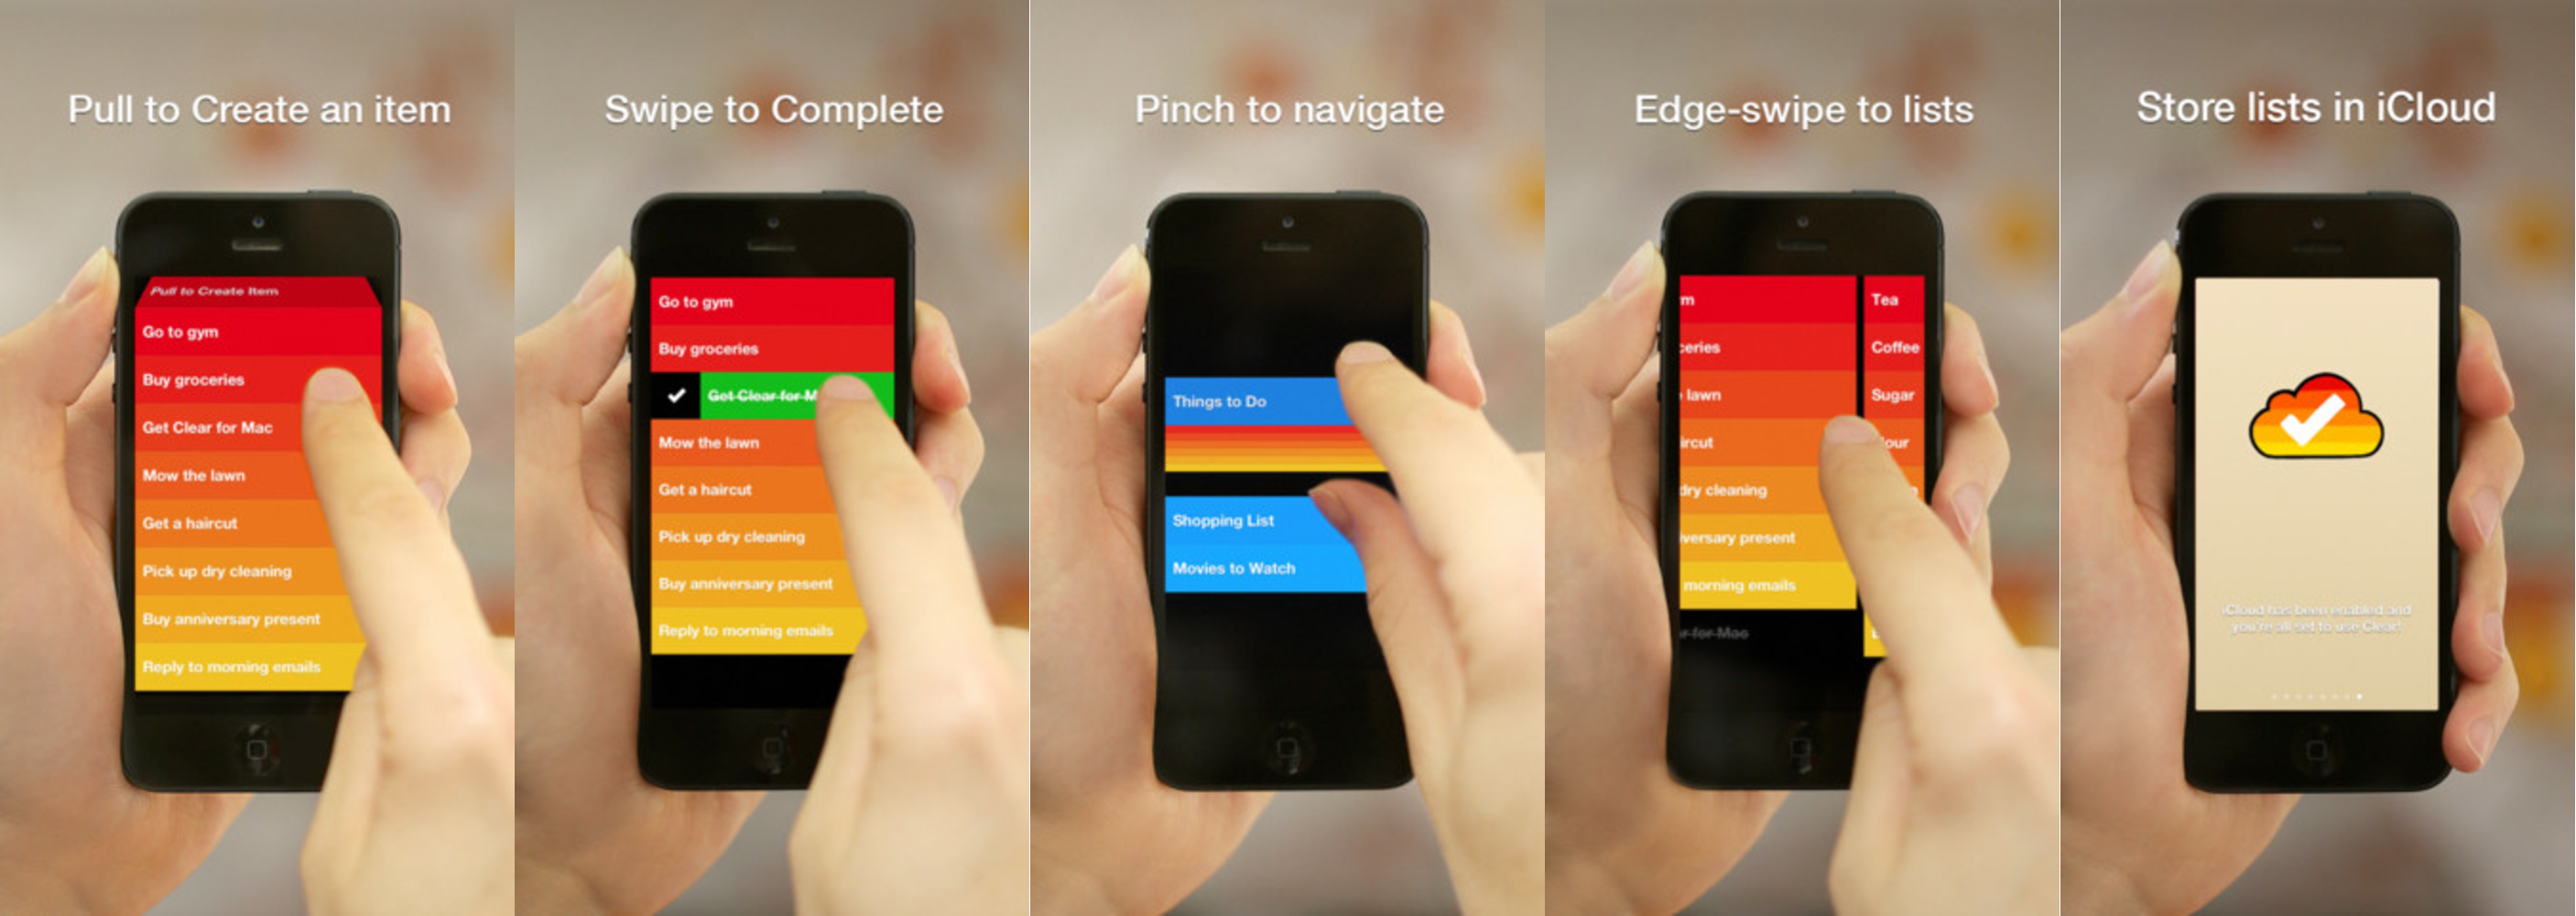
\includegraphics[width=0.9\textwidth]{resources/clear.pdf}
	\caption[Clear]{Clear}
\end{figure}

\textbf{Remember the milk.} \url{http://www.rememberthemilk.com/} Remember the milk offers a lot of GTD functionality: tag clouds, custom task lists, geo location, Gmail extension, Google Calendar integration, etc.

\begin{figure}
   \centering
	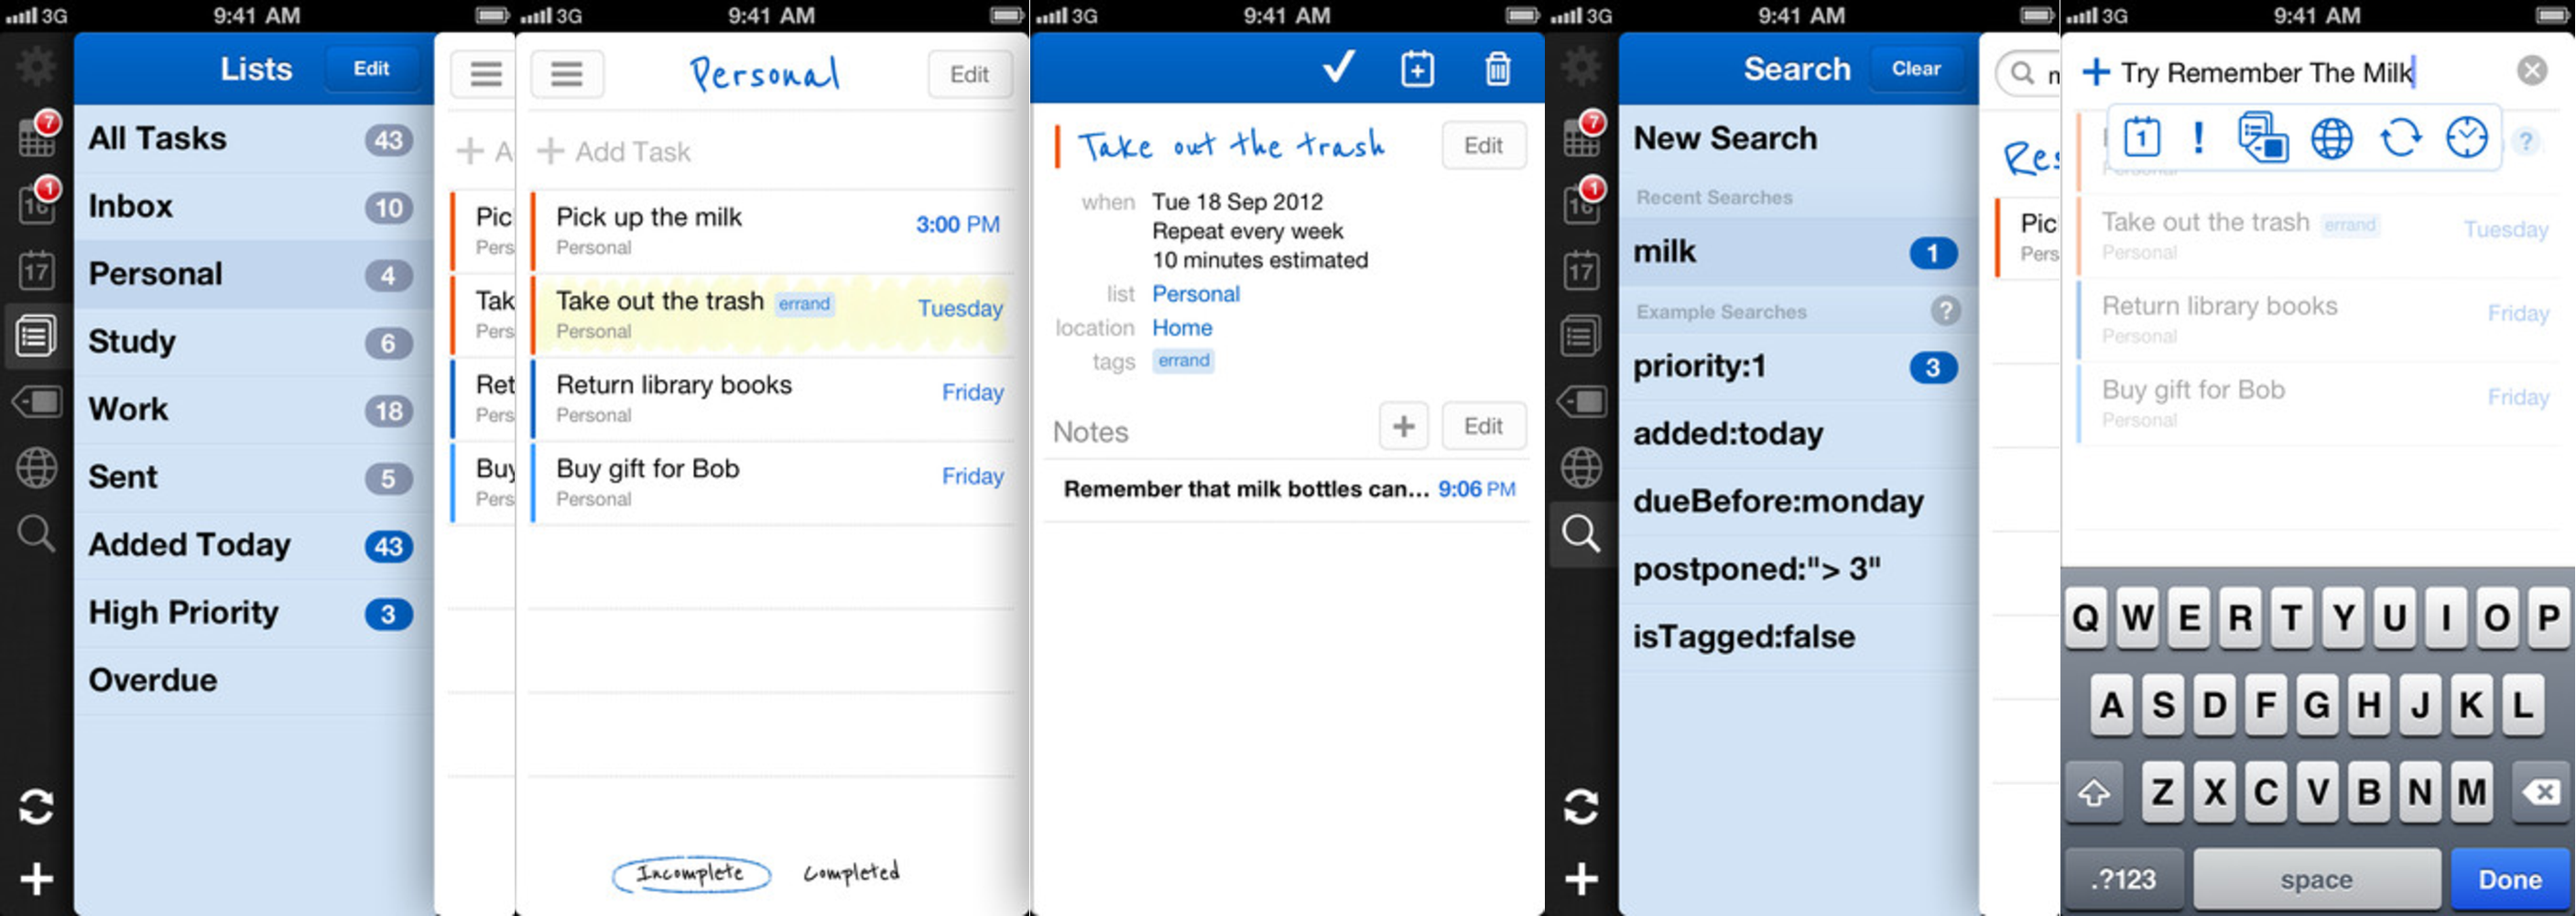
\includegraphics[width=0.9\textwidth]{resources/remember-the-milk.pdf}
	\caption[Remember the milk]{Remember the milk}
\end{figure}

\textbf{Wunderlist 2.} \url{https://www.wunderlist.com} Wunderlist 2 comes with a number of features: online syncing, filtered lists, and Facebook integration, collaboration. The design spans across the multitude of different devices Wunderlist works on, giving it a single, unified interface.

\begin{figure}
   \centering
	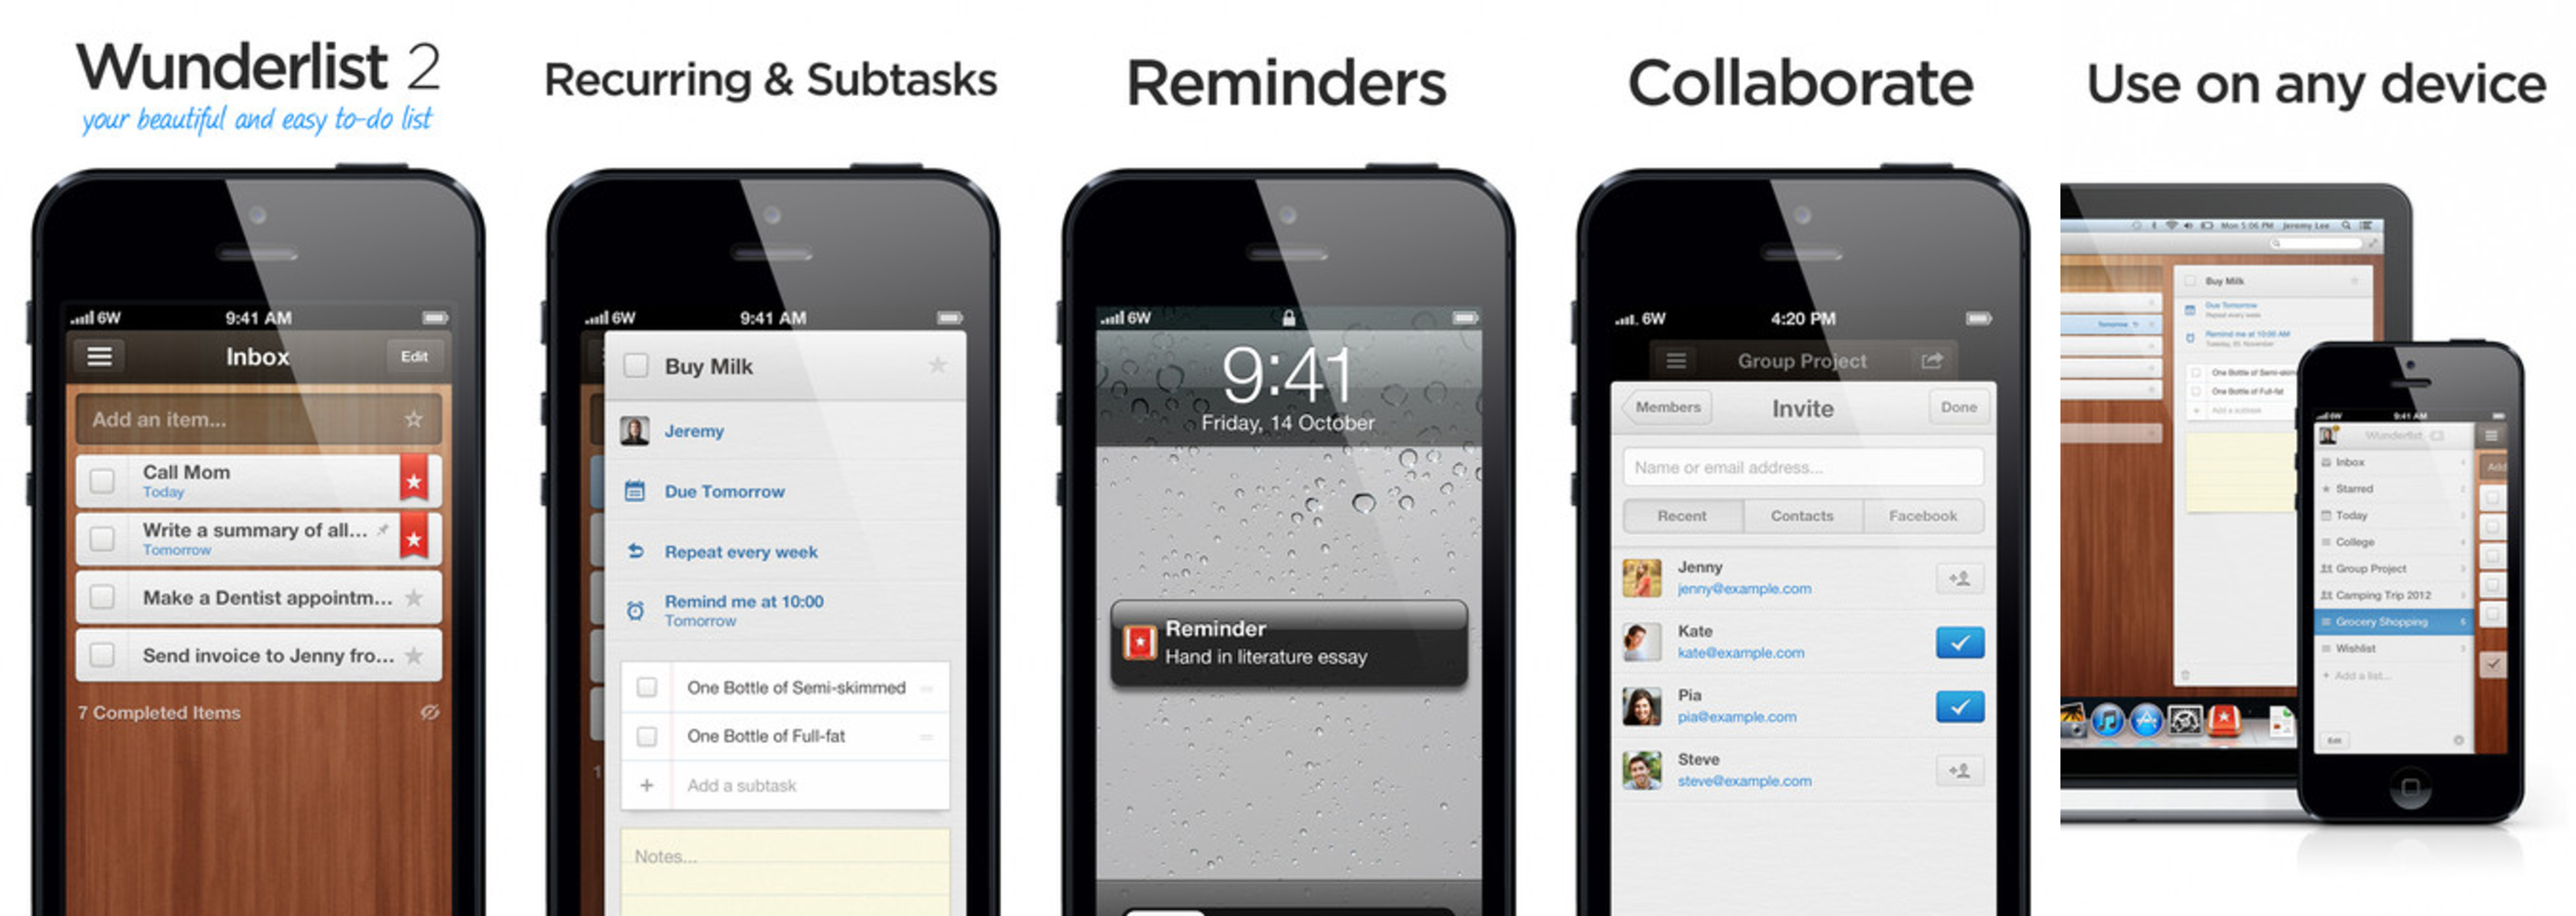
\includegraphics[width=0.9\textwidth]{resources/wunderlist.pdf}
	\caption[Wunderlist]{Wunderlist}
\end{figure}

\textbf{Flow.} \url{http://www.getflow.com/} Flow provides all the collaboration tools needed to manage a project (files, deadlines, tasks and discussion) online in one centralized place for everyone. It allows to discuss projects, set deadlines, take notes, and keep everyone on the same page online, even when they're out of the office.

\begin{figure}
   \centering
	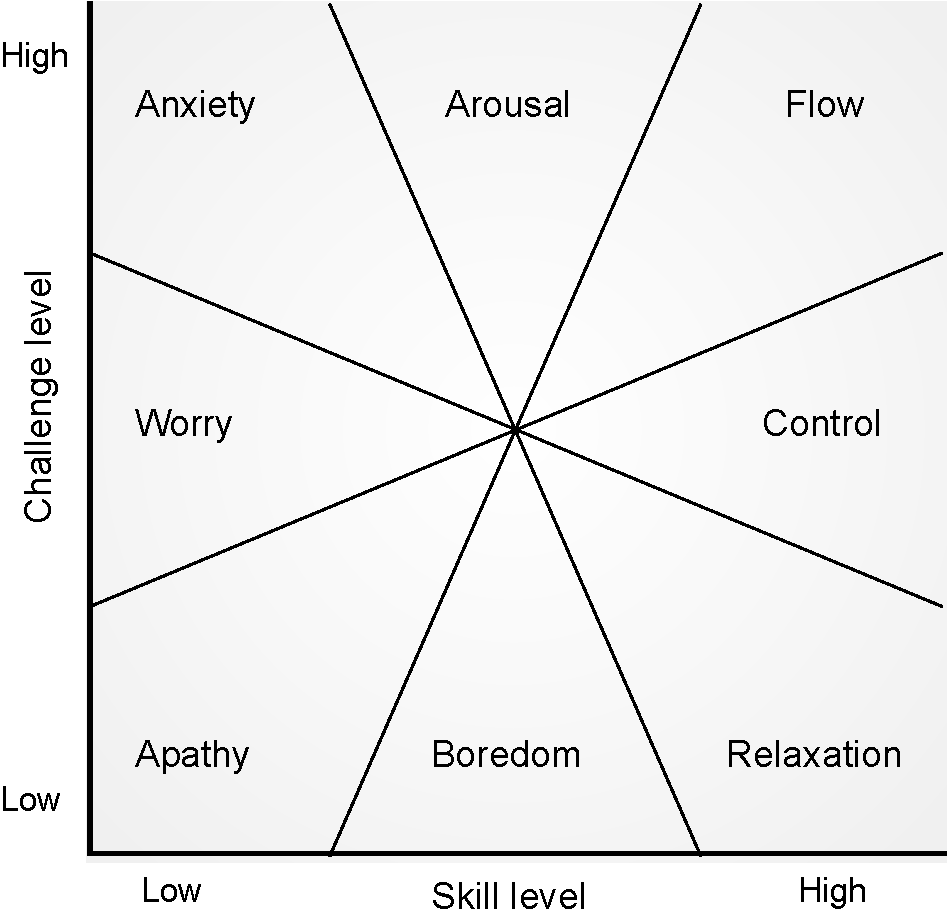
\includegraphics[width=0.9\textwidth]{resources/flow.pdf}
	\caption[Flow]{Flow}
\end{figure}

\textbf{Things.} \url{http://culturedcode.com/things/iphone/} Things features a daily review to plan a day on the go: to-dos that are scheduled for today automatically appear at the top of Today list, together with to-dos that have become due; instant action to find the right tasks for the current context using tags; predefined lists, such as ``today", ``next", ``scheduled", ``someday".

\begin{figure}
   \centering
	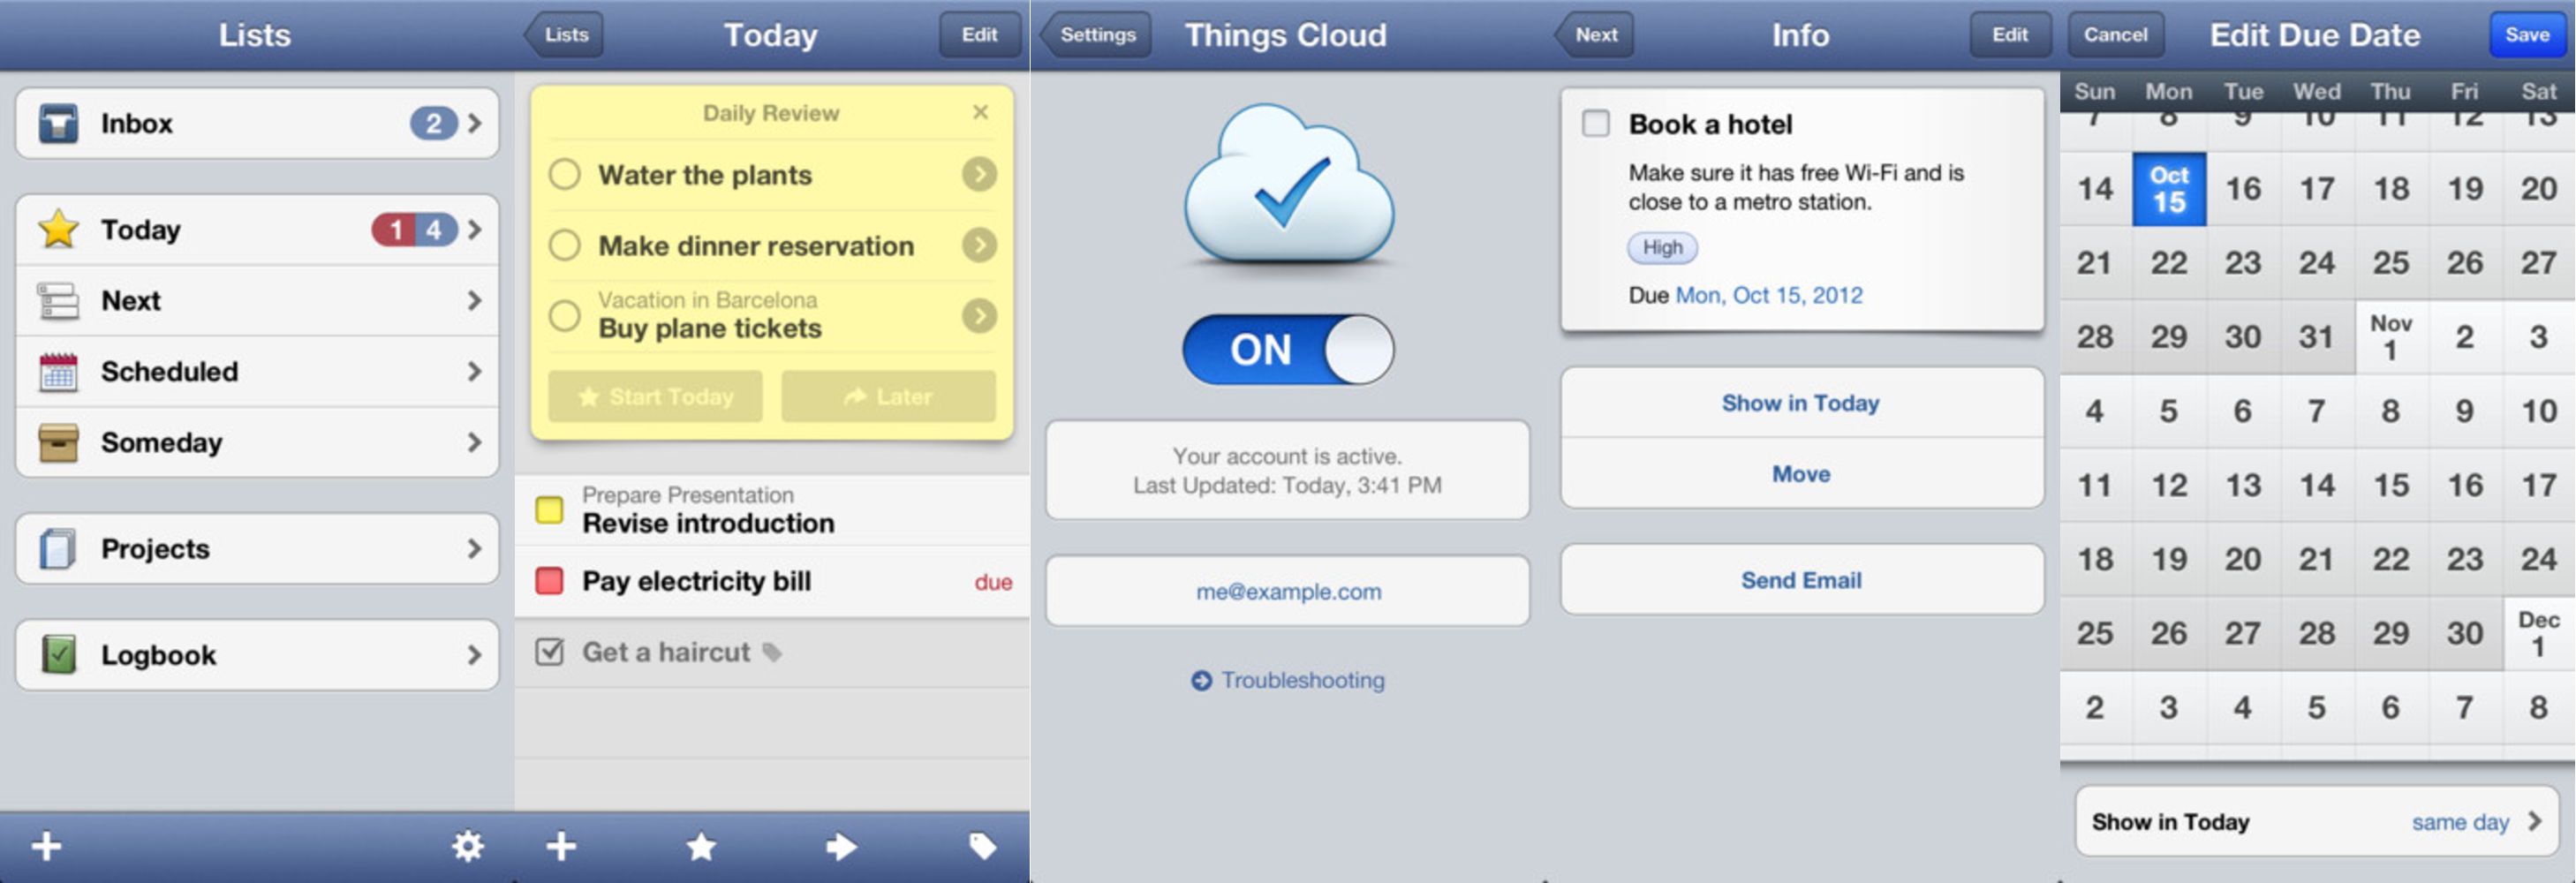
\includegraphics[width=0.9\textwidth]{resources/things.pdf}
	\caption[Things]{Things}
\end{figure}

\section{Game mechanics in use}

Most of the listed applications made a different approach to these mechanics. But only one application tried to develop an emotional connection to a person. It is Carrot, which uses natural language and colour-coded emotions in order to response to actions of a person. If a person didn’t achieve anything in a period of time, Carrot becomes angry. In addition, this application used the most of introduced game mechanics (see table \ref{tab:appsandmech}).

Achievement definition: A virtual or physical representation of having accomplished something. These are often viewed as rewards in and of themselves.
Pride definition: the feeling of ownership and joy at an accomplishment.

\begin{longtable}{|p{0.3\linewidth}|p{0.5\linewidth}|}
\caption{Popular applications and used game mechanics}
\label{tab:appsandmech}\\
\hline
\bf Application &  \bf Game Mechanics \\
\hline
\endhead
Habit List & Achievement, pride, avoidance \\
\hline
Carrot & Cascading Information Theory, pride, avoidance, achievement, progression dynamic \\
\hline
Clear & Cascading Information Theory, Achievement \\
\hline
Remember the milk & Achievement \\
\hline
Wunderlist 2 & Achievement, pride \\
\hline
Flow & Achievement, communal discovery \\
\hline
Things & Achievement\\
\hline
\end{longtable}

Avoidance definition:  the act of inducing player behavior not by giving a reward, but by not instituting a punishment. Produces consistent level of activity, timed around the schedule.

Communal Discovery definition: The game dynamic wherein an entire community is rallied to work together to solve a riddle, a problem or a challenge. Immensely viral and very fun.
Cascading Information Theory definition: The theory that information should be released in the minimum possible snippets to gain the appropriate level of understanding at each point during a game narrative.

Progression dynamic definition: this is a dynamic in which success is granularly displayed and measured through the process of completing itemised tasks.

\section{What to learn from productivity apps}

Summarizing the conducted results, the following list of requirements for successful productivity application was made:
\begin{compactitem}
\item ``Achievement" game mechanics supports desire to perform tasks
\item ``Pride" game mechanics supports retention of joy from executed tasks
\item ``Avoidance" game mechanics helps a person return to application
\item ``Cascading Information Theory" allows to introduce difficult concepts of GTD (Getting Things Done) and increase a person’s activity in the application
\item ``Communal Discovery" is used in collaborative tasks / task delegation
\item ``Progression Dynamic" helps visualise improvement and progress to a goal.
\end{compactitem}

Techniques used in animation to create believable characters can help to establish an emotional connection to the person.
